% Options for packages loaded elsewhere
\PassOptionsToPackage{unicode}{hyperref}
\PassOptionsToPackage{hyphens}{url}
\PassOptionsToPackage{dvipsnames,svgnames,x11names}{xcolor}
%
\documentclass[
  letterpaper,
  DIV=11,
  numbers=noendperiod]{scrartcl}

\usepackage{amsmath,amssymb}
\usepackage{iftex}
\ifPDFTeX
  \usepackage[T2A]{fontenc}
  \usepackage[utf8]{inputenc}
  \usepackage{textcomp} % provide euro and other symbols
\else % if luatex or xetex
  \usepackage{unicode-math}
  \defaultfontfeatures{Scale=MatchLowercase}
  \defaultfontfeatures[\rmfamily]{Ligatures=TeX,Scale=1}
\fi
\usepackage{lmodern}
\ifPDFTeX\else  
    % xetex/luatex font selection
  \setmainfont[]{CMU Serif}
  \setsansfont[]{CMU Serif}
  \setmonofont[]{CMU Serif}
\fi
% Use upquote if available, for straight quotes in verbatim environments
\IfFileExists{upquote.sty}{\usepackage{upquote}}{}
\IfFileExists{microtype.sty}{% use microtype if available
  \usepackage[]{microtype}
  \UseMicrotypeSet[protrusion]{basicmath} % disable protrusion for tt fonts
}{}
\makeatletter
\@ifundefined{KOMAClassName}{% if non-KOMA class
  \IfFileExists{parskip.sty}{%
    \usepackage{parskip}
  }{% else
    \setlength{\parindent}{0pt}
    \setlength{\parskip}{6pt plus 2pt minus 1pt}}
}{% if KOMA class
  \KOMAoptions{parskip=half}}
\makeatother
\usepackage{xcolor}
\setlength{\emergencystretch}{3em} % prevent overfull lines
\setcounter{secnumdepth}{-\maxdimen} % remove section numbering
% Make \paragraph and \subparagraph free-standing
\ifx\paragraph\undefined\else
  \let\oldparagraph\paragraph
  \renewcommand{\paragraph}[1]{\oldparagraph{#1}\mbox{}}
\fi
\ifx\subparagraph\undefined\else
  \let\oldsubparagraph\subparagraph
  \renewcommand{\subparagraph}[1]{\oldsubparagraph{#1}\mbox{}}
\fi


\providecommand{\tightlist}{%
  \setlength{\itemsep}{0pt}\setlength{\parskip}{0pt}}\usepackage{longtable,booktabs,array}
\usepackage{calc} % for calculating minipage widths
% Correct order of tables after \paragraph or \subparagraph
\usepackage{etoolbox}
\makeatletter
\patchcmd\longtable{\par}{\if@noskipsec\mbox{}\fi\par}{}{}
\makeatother
% Allow footnotes in longtable head/foot
\IfFileExists{footnotehyper.sty}{\usepackage{footnotehyper}}{\usepackage{footnote}}
\makesavenoteenv{longtable}
\usepackage{graphicx}
\makeatletter
\def\maxwidth{\ifdim\Gin@nat@width>\linewidth\linewidth\else\Gin@nat@width\fi}
\def\maxheight{\ifdim\Gin@nat@height>\textheight\textheight\else\Gin@nat@height\fi}
\makeatother
% Scale images if necessary, so that they will not overflow the page
% margins by default, and it is still possible to overwrite the defaults
% using explicit options in \includegraphics[width, height, ...]{}
\setkeys{Gin}{width=\maxwidth,height=\maxheight,keepaspectratio}
% Set default figure placement to htbp
\makeatletter
\def\fps@figure{htbp}
\makeatother

\KOMAoption{captions}{tablesignature}
\usepackage{csquotes}
\usepackage[authordate, abbreviate = true, date = year, autocite=inline, backref = true]{biblatex-chicago}
\makeatletter
\makeatother
\makeatletter
\makeatother
\makeatletter
\@ifpackageloaded{caption}{}{\usepackage{caption}}
\AtBeginDocument{%
\ifdefined\contentsname
  \renewcommand*\contentsname{Table of contents}
\else
  \newcommand\contentsname{Table of contents}
\fi
\ifdefined\listfigurename
  \renewcommand*\listfigurename{List of Figures}
\else
  \newcommand\listfigurename{List of Figures}
\fi
\ifdefined\listtablename
  \renewcommand*\listtablename{List of Tables}
\else
  \newcommand\listtablename{List of Tables}
\fi
\ifdefined\figurename
  \renewcommand*\figurename{Figure}
\else
  \newcommand\figurename{Figure}
\fi
\ifdefined\tablename
  \renewcommand*\tablename{Table}
\else
  \newcommand\tablename{Table}
\fi
}
\@ifpackageloaded{float}{}{\usepackage{float}}
\floatstyle{ruled}
\@ifundefined{c@chapter}{\newfloat{codelisting}{h}{lop}}{\newfloat{codelisting}{h}{lop}[chapter]}
\floatname{codelisting}{Listing}
\newcommand*\listoflistings{\listof{codelisting}{List of Listings}}
\makeatother
\makeatletter
\@ifpackageloaded{caption}{}{\usepackage{caption}}
\@ifpackageloaded{subcaption}{}{\usepackage{subcaption}}
\makeatother
\makeatletter
\@ifpackageloaded{tcolorbox}{}{\usepackage[skins,breakable]{tcolorbox}}
\makeatother
\makeatletter
\@ifundefined{shadecolor}{\definecolor{shadecolor}{rgb}{.97, .97, .97}}
\makeatother
\makeatletter
\makeatother
\makeatletter
\makeatother
\ifLuaTeX
\usepackage[bidi=basic]{babel}
\else
\usepackage[bidi=default]{babel}
\fi
\babelprovide[main,import]{english}
% get rid of language-specific shorthands (see #6817):
\let\LanguageShortHands\languageshorthands
\def\languageshorthands#1{}
\ifLuaTeX
  \usepackage{selnolig}  % disable illegal ligatures
\fi
\usepackage[]{biblatex}
\addbibresource{bibliography.bib}
\usepackage{csquotes}
\IfFileExists{bookmark.sty}{\usepackage{bookmark}}{\usepackage{hyperref}}
\IfFileExists{xurl.sty}{\usepackage{xurl}}{} % add URL line breaks if available
\urlstyle{same} % disable monospaced font for URLs
\hypersetup{
  pdftitle={Student dropout analysis based on previously acquired educational achievements: A case of the University of Portalegre},
  pdfauthor={Izeldeen Nedal Yunis Al Fraijat; Danat Semeneev; Ieva Žube; Pankaj Chettri; Kristaps Eglītis},
  pdflang={en},
  pdfkeywords={AA1, AA2},
  colorlinks=true,
  linkcolor={blue},
  filecolor={Maroon},
  citecolor={Blue},
  urlcolor={Blue},
  pdfcreator={LaTeX via pandoc}}

\title{Student dropout analysis based on previously acquired educational
achievements: A case of the University of Portalegre}
\usepackage{etoolbox}
\makeatletter
\providecommand{\subtitle}[1]{% add subtitle to \maketitle
  \apptocmd{\@title}{\par {\large #1 \par}}{}{}
}
\makeatother
\subtitle{Business Analysis, Business Informatics Ms, Fall 2023.}
\author{Izeldeen Nedal Yunis Al Fraijat \and Danat Semeneev \and Ieva
Žube \and Pankaj Chettri \and Kristaps Eglītis\footnote{Rīga Technical
  University}}
\date{2023-12-13}

\begin{document}
\maketitle
\begin{abstract}
.
\end{abstract}
\ifdefined\Shaded\renewenvironment{Shaded}{\begin{tcolorbox}[sharp corners, borderline west={3pt}{0pt}{shadecolor}, frame hidden, boxrule=0pt, interior hidden, enhanced, breakable]}{\end{tcolorbox}}\fi

\hypertarget{abstract}{%
\subsection{Abstract}\label{abstract}}

In the world of education, a person's path is often depicted as a linear
progression, where students follow a predefined journey from
kindergarten to graduation. However, the reality is far more complex.
There could be various reasons that emerge during the study program that
led students to deviate from this path. These students might encounter
different challenges, circumstances, or a lack of proper resources that
have led them to drop out of university.

In this dataset provided to us, we will delve deeper into understanding
the reasons why students have dropped out of the university. We will
leverage our social knowledge to comprehend the factors that influenced
their decision to drop out and work to prevent such occurrences if the
issues are within the university's purview. Our goal is to propose
solutions and their support so that high schools could facilitate and
secure students' educational journeys. We construct the best basic model
that predicts the results with 73\% balanced precision recall. We
provide the recommedatons based on findings and define auxiliary
requisite data to further our research in the future.

\hypertarget{introduction}{%
\section{Introduction}\label{introduction}}

Starting from preliminary school we are told that having an education is
very important for your future or that without higher education your job
possibilities are going to be very limited. While primary education is
mandatory, having higher education is not. There are, however, many
reasons for which people may want to pursue higher education. According
to studies, many factors are materialistic, the most important factor
for pursuing higher education is job acquisition
\autocite{knutsen_motivation_2011}. Some other factors may include
increased income in the existing job, improved work conditions or
increased ability for retirement. Of course, other, more intrisic
factors include seeking for additional knowledge or self-fulfillment
\autocite{cortes_factors_2023}. There are also factors like meeting new
friends, improving social interaction skills or just wanting to make a
difference in the world. Of course factors that cannot be ignored are
social pressure \autocite{temple_factors_2009}, meaning that having
friends that want to pursue higher education can influence ones own
decision or influence of family members. However, there are people that
discontinue their studies prematurely and we are interested to learn
what the reasons for such a decision could be. Based on the study and
datasets that we used for our research there are multiple factors that
influence dropping out.

Nevertheless, pursuing higher education and actually getting the degree
has some tangible benefits. According to an OECD -- Education at a
Glance 2019 research paper \autocite{oecd_education_2019}.

\begin{quote}
\enquote{On average across OECD countries, adults with a short-cycle
tertiary degree earn 20\% more than adults with upper secondary
education. The earnings advantage increases to 44\% for those with a
bachelor's degree and to 91\% for those with a master's or doctoral
degree.}
\end{quote}

With this in mind, it is important for government and educational
institutions to ensure high level of graduates in society to ensure
economic growth and overall increase in well-being. To measure the
success of this goal, it is important to set KPI's, track them and make
educated conclusions on what needs to be done or is being done right to
reach the goal of higher educated society.

\hypertarget{sec-kpi}{%
\subsection{Target Metrics and KPI}\label{sec-kpi}}

In this particular case, KPI's will be chosen based on datasets of
Portugese High Schools but most likely data can be generalised, atleast
for Europe, as the region and sociodemographics are not so different.
Even though there are many factors that influence the success of
graduation, only factors that can be proven by government and
educational institutions will be chosen. In order to thwart
embezzlement, indicators should be restricted in magnitude and difficult
to falsify or manipulate. After rigorous analysis, we propose the
following KPIs.

\begin{enumerate}
\def\labelenumi{\alph{enumi}.}
\tightlist
\item
  \textbf{Student grade improvement compared to support}. Based on the
  dataset, students who had support had 3x lower dropout rates than
  students that didn't have. While it is not practical to allocate
  higher amount of money for studying that itself does not generate
  value, it scoops that it at least a sizeable parts of the dropout
  students could be held from leaving with a relatively small aid that
  would make the benefits of studies outweigh those of working/etc.
  Leaving is commonly associated with very poor grades (otherwise, even
  a morally disinterested student would opt to formally remain in the
  university until they are asked to leave due to poor performance).
  Since a person with infinitesimal grades is a clear candidate for
  dropping out, one should identify those students with abrupt downward
  grade dynamics and quench this. In the proposed KPI, the
  \((grade)_{i}\) is the mean relative grade change for student \(j\)
  over all their courses at university i at moment t, and the assistance
  is the mean aid per student (can be 0). If there are no students on
  their way down , the KPI is guaranteed to be positive.
\end{enumerate}

\[KPI_{1, i,t} =  \frac{|\Delta(\bar{grade})_i|}{ (\bar{assistance}_i)}\]
This does not depend on the number of courses, because the courses are
themselves different difficulties, the important thing that the
university (the students too) should look after in this regard, that the
situation with grades does drastically deteriorate over time.

\begin{enumerate}
\def\labelenumi{\alph{enumi}.}
\item
  \textbf{Institutional Improvements}. Although volatile and subjective,
  as one of the metrics (not KPIs, since it is more difficult to tie
  this to specific redresses) there could be a longitudinal survey about
  one's satisfaction with the studies and programme in general in the
  fashion of a job an exit or quasi-exit interview (when a person does
  not leave actually, but they are still invited to answer the questions
  as if they would be leaving). This would allow to track the scale of
  dropouts due to frustration with the programme (not engaging enough).
\item
  \textbf{Relative changes in student's grades}. Datasets tell us that
  the higher the average grade, the lower the dropout rate. Usually
  students that have low grades are uninterested in the subjects which
  could be due to having chosen not the right program for them or that
  the way lectures and information is presented is uninteresting or
  outdated. Either way this can be improved. Increasing the possibility
  that the student has chosen the right program for him can be done by
  introducing more \enquote{open days} in higher education institutions
  and having more upfront information about what can be expected from
  programs. The overall lecture performance can be improved by taking
  more time to have up-to-date information presented and teachers having
  decent motivation of teaching students. This can be achieved by
  increasing teacher salaries and institutions having more control over
  teachers and information they present to students.
\end{enumerate}

All these metrics are still vulnerable to misrepresentation, but it is
inevitable given the freedom the universities enjoy in managing their
study programmes. Still, any manipulation of this metrics can only be
temporary and thus is also not in the best interest of the university.

\hypertarget{sec-eda}{%
\subsection{Exploratory Data Analysis}\label{sec-eda}}

\hypertarget{descriptive-statistics}{%
\subsubsection{Descriptive Statistics}\label{descriptive-statistics}}

As we have checked, the dataset does not have zero values, so there is
nothing to purge inside it. Later on, we get the basic descriptive
statistics, shown below in\\
Tables~\ref{tbl-descstat-3}, \ref{tbl-descstat-1}, \ref{tbl-descstat-2}, \ref{tbl-descstat-4}, \ref{tbl-descstat-5}, \ref{tbl-descstat-6}, \ref{tbl-descstat-7}

\hypertarget{tbl-descstat-1}{}
\begin{longtable}[]{@{}lrrrrr@{}}
\toprule\noalign{}
& Mari. stat. & Appl. mode. & Appl. orde. & Cour. & Dayt. atte. \\
\midrule\noalign{}
\endfirsthead
\toprule\noalign{}
& Mari. stat. & Appl. mode. & Appl. orde. & Cour. & Dayt. atte. \\
\midrule\noalign{}
\endhead
\bottomrule\noalign{}
\endlastfoot
count & 4424 & 4424 & 4424 & 4424 & 4424 \\
mean & 1.18 & 18.67 & 1.73 & 8856.64 & 0.89 \\
std & 0.61 & 17.48 & 1.31 & 2063.57 & 0.31 \\
min & 1 & 1 & 0 & 33 & 0 \\
25\% & 1 & 1 & 1 & 9085 & 1 \\
50\% & 1 & 17 & 1 & 9238 & 1 \\
75\% & 1 & 39 & 2 & 9556 & 1 \\
max & 6 & 57 & 9 & 9991 & 1 \\
\caption{\label{tbl-descstat-1}Descriptive statistics}\tabularnewline
\end{longtable}

\hypertarget{tbl-descstat-2}{}
\begin{longtable}[]{@{}lrrrrr@{}}
\toprule\noalign{}
& Prev. qual. & Prev. qual. (gra. & Naci. & Moth. qual. & Fath. qual. \\
\midrule\noalign{}
\endfirsthead
\toprule\noalign{}
& Prev. qual. & Prev. qual. (gra. & Naci. & Moth. qual. & Fath. qual. \\
\midrule\noalign{}
\endhead
\bottomrule\noalign{}
\endlastfoot
count & 4424 & 4424 & 4424 & 4424 & 4424 \\
mean & 4.58 & 132.61 & 1.87 & 19.56 & 22.28 \\
std & 10.22 & 13.19 & 6.91 & 15.6 & 15.34 \\
min & 1 & 95 & 1 & 1 & 1 \\
25\% & 1 & 125 & 1 & 2 & 3 \\
50\% & 1 & 133.1 & 1 & 19 & 19 \\
75\% & 1 & 140 & 1 & 37 & 37 \\
max & 43 & 190 & 109 & 44 & 44 \\
\caption{\label{tbl-descstat-2}Descriptive statistics
(cont'd)}\tabularnewline
\end{longtable}

\hypertarget{tbl-descstat-3}{}
\begin{longtable}[]{@{}llllll@{}}
\toprule\noalign{}
& Mother\textquotesingle s occupation & Father\textquotesingle s
occupation & Admission grade & Displaced & Educational special needs \\
\midrule\noalign{}
\endfirsthead
\toprule\noalign{}
& Mother\textquotesingle s occupation & Father\textquotesingle s
occupation & Admission grade & Displaced & Educational special needs \\
\midrule\noalign{}
\endhead
\bottomrule\noalign{}
\endlastfoot
count & 4424.00 & 4424.00 & 4424.00 & 4424.00 & 4424.00 \\
mean & 10.96 & 11.03 & 126.98 & 0.55 & 0.01 \\
std & 26.42 & 25.26 & 14.48 & 0.50 & 0.11 \\
min & 0.00 & 0.00 & 95.00 & 0.00 & 0.00 \\
25\% & 4.00 & 4.00 & 117.90 & 0.00 & 0.00 \\
50\% & 5.00 & 7.00 & 126.10 & 1.00 & 0.00 \\
75\% & 9.00 & 9.00 & 134.80 & 1.00 & 0.00 \\
max & 194.00 & 195.00 & 190.00 & 1.00 & 1.00 \\
\caption{\label{tbl-descstat-3}Descriptive statistics
(cont'd)}\tabularnewline
\end{longtable}

\begin{verbatim}
'Curricular units 2nd sem (enrolled), Curricular units 2nd sem (evaluations), Curricular units 2nd sem (approved), Curricular units 2nd sem (grade)'
\end{verbatim}

\hypertarget{tbl-descstat-4}{}
\begin{longtable}[]{@{}llllll@{}}
\toprule\noalign{}
\endfirsthead
\endhead
\bottomrule\noalign{}
\endlastfoot
count & 4424 & 4424 & 4424 & 4424 & 4424 \\
mean & 0.11 & 0.88 & 0.35 & 0.25 & 23.27 \\
std & 0.32 & 0.32 & 0.48 & 0.43 & 7.59 \\
min & 0 & 0 & 0 & 0 & 17 \\
25\% & 0 & 1 & 0 & 0 & 19 \\
50\% & 0 & 1 & 0 & 0 & 20 \\
75\% & 0 & 1 & 1 & 0 & 25 \\
max & 1 & 1 & 1 & 1 & 70 \\
\caption{\label{tbl-descstat-4}Descriptive statistics (cont'd). Columns,
left-to-right: Debtor, Tuition fees up to date, Gender, Scholarship
holder, Age at enrollment}\tabularnewline
\end{longtable}

\hypertarget{tbl-descstat-5}{}
\begin{longtable}[]{@{}lllll@{}}
\toprule\noalign{}
\endfirsthead
\endhead
\bottomrule\noalign{}
\endlastfoot
count & 4424 & 4424 & 4424 & 4424 \\
mean & 0.02 & 0.71 & 6.27 & 8.3 \\
std & 0.16 & 2.36 & 2.48 & 4.18 \\
min & 0 & 0 & 0 & 0 \\
25\% & 0 & 0 & 5 & 6 \\
50\% & 0 & 0 & 6 & 8 \\
75\% & 0 & 0 & 7 & 10 \\
max & 1 & 20 & 26 & 45 \\
\caption{\label{tbl-descstat-5}Descriptive statistics (cont'd). Columns
International, Curricular units 1st sem (credited), Curricular units 1st
sem (enrolled), Curricular units 1st sem (evaluations).}\tabularnewline
\end{longtable}

\hypertarget{tbl-descstat-6}{}
\begin{longtable}[]{@{}lllll@{}}
\toprule\noalign{}
\endfirsthead
\endhead
\bottomrule\noalign{}
\endlastfoot
count & 4424 & 4424 & 4424 & 4424 \\
mean & 4.71 & 10.64 & 0.14 & 0.54 \\
std & 3.09 & 4.84 & 0.69 & 1.92 \\
min & 0 & 0 & 0 & 0 \\
25\% & 3 & 11 & 0 & 0 \\
50\% & 5 & 12.29 & 0 & 0 \\
75\% & 6 & 13.4 & 0 & 0 \\
max & 26 & 18.88 & 12 & 19 \\
\caption{\label{tbl-descstat-6}Descriptive statistics (cont'd). Columns
Curricular units 1st sem (approved), Curricular units 1st sem (grade),
Curricular units 1st sem (without evaluations), Curricular units 2nd sem
(credited)'}\tabularnewline
\end{longtable}

\hypertarget{tbl-descstat-7}{}
\begin{longtable}[]{@{}lllll@{}}
\toprule\noalign{}
\endfirsthead
\endhead
\bottomrule\noalign{}
\endlastfoot
count & 4424 & 4424 & 4424 & 4424 \\
mean & 6.23 & 8.06 & 4.44 & 10.23 \\
std & 2.2 & 3.95 & 3.01 & 5.21 \\
min & 0 & 0 & 0 & 0 \\
25\% & 5 & 6 & 2 & 10.75 \\
50\% & 6 & 8 & 5 & 12.2 \\
75\% & 7 & 10 & 6 & 13.33 \\
max & 23 & 33 & 20 & 18.57 \\
\caption{\label{tbl-descstat-7}Descriptive statistics (cont'd).
Curricular units 2nd sem (enrolled), Curricular units 2nd sem
(evaluations), Curricular units 2nd sem (approved), Curricular units 2nd
sem (grade)'}\tabularnewline
\end{longtable}

The students are from multiple countries, but the overwhelming majority
of the students are from Portugal. It would be interesting to see how
the students' admission grade depends on their previous qualification in
their home countries, but the samples are scarce. Many students from
abroad are from the Overseas Territories where it's more challenging to
get comparable education. However, they and inland Portugal students
were naturally given some exemptions, as the dataset states \footnote{Link
  to the dataset description:
  \url{https://archive.ics.uci.edu/dataset/697/predict+students+dropout+and+academic+success}}.
\footnote{Notably, the authors did not specify all categories of
  students even in the description to the dataset, so it can be regarded
  as one of \enquote*{issues} of the dataset that it can be challenging
  to fully interpret the feature store.}

For example, the students admitted per Ordance no. 854 \footnote{Link to
  the source document:
  \url{https://dre.tretas.org/dre/106607/portaria-854-B-99-de-4-de-outubro}}
were not required to demonstrate the proof of their validity since their
received a diploma in secondary education administered in Portuguese
(Angola, East Timor, Mozambique, Guinea Equatorial). Students admitted
per Ordnance no. 533 \footnote{Link to the source document:
  \url{https://dre.tretas.org/dre/104726/portaria-533-A-99-de-22-de-julho}}
were from another university in Portugal with overlapping courses
covered recently enough so they were not required to repeat them.
Finally, those admitted per Ordnance no. 612 \footnote{Link to the
  source document:
  \url{https://dre.tretas.org/dre/51542/portaria-612-93-de-29-de-junho}}
came from other countries but had comparable material in their studies
and so their points were recalculated with some amortization.

\hypertarget{data-visualizations}{%
\subsubsection{Data Visualizations}\label{data-visualizations}}

\begin{figure}

{\centering 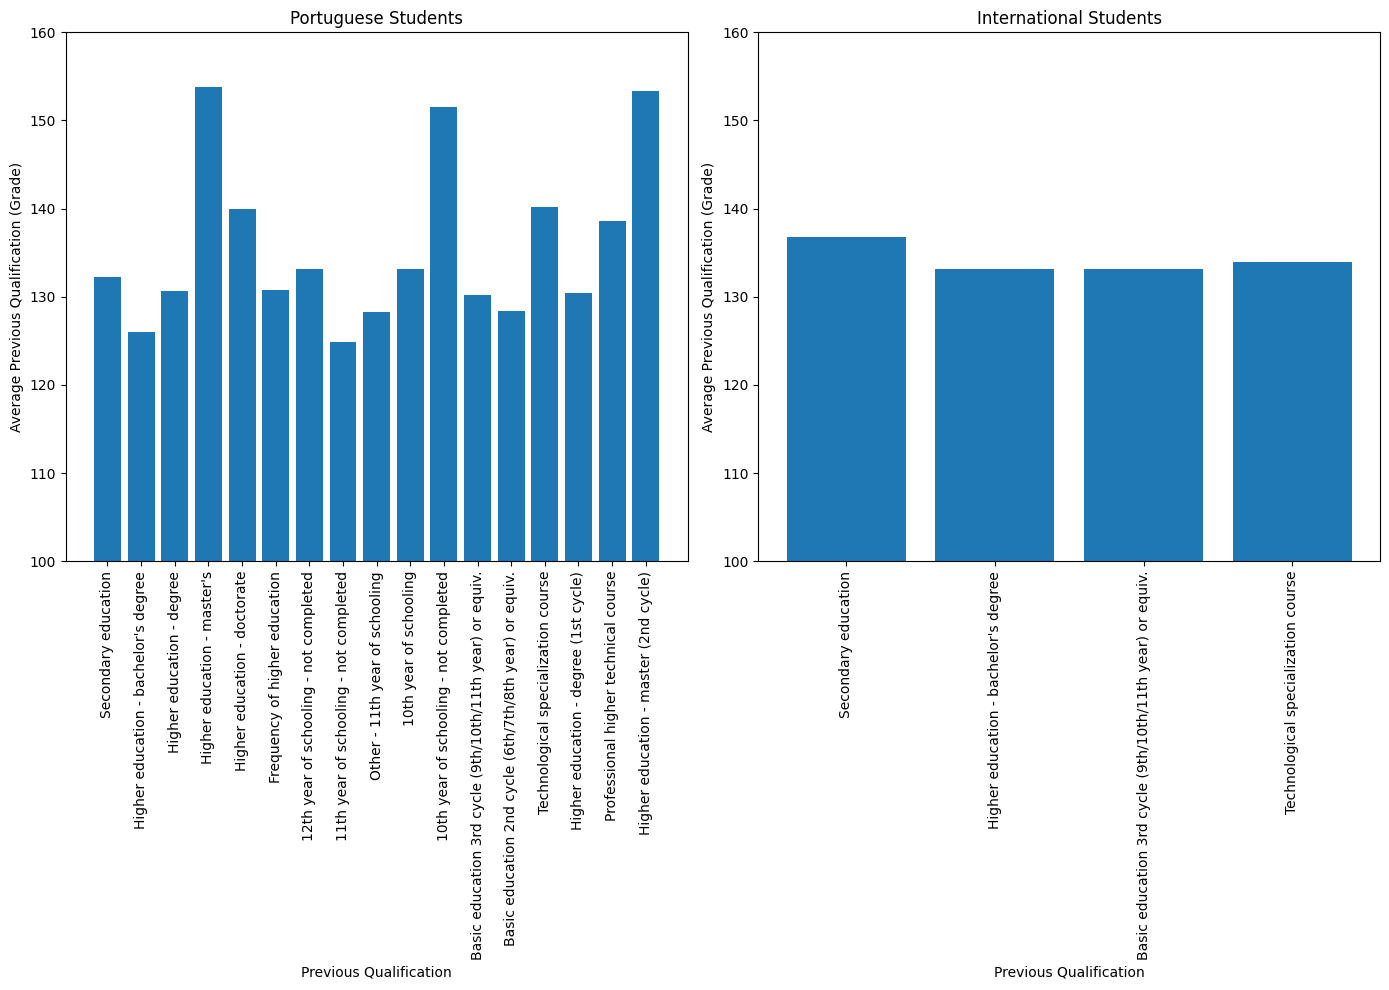
\includegraphics{report_AzadhdhinNedalYunisAlFraijat_files/figure-pdf/fig-education-output-1.png}

}

\caption{\label{fig-education}Relative graduation points for students
with different education backgrounds}

\end{figure}

Due to class imbalance , the variability for the Portuguese students is
much higher, and while the 3 categories (see Figure~\ref{fig-education})
with highest grades are natural, i. e. doctors, masters as higher
education, the 3rd is unintuitive (the 10 classes) and we tend to
explain it as self-selection and high correlation with other indicators
(those entering the university in the 10th grade are more motivated then
dwelling in schools in 11th and 12th grades).

Also, there is a drastic imbalance over yet another crucial factor: age.
Students of age are far less ubiquitous, can have far more incentives to
abandon studies and smaller potential for apprehension of material.
Indeed, this is clearly shown on the next graph \ref{fig-age-distr}

\begin{figure}

{\centering 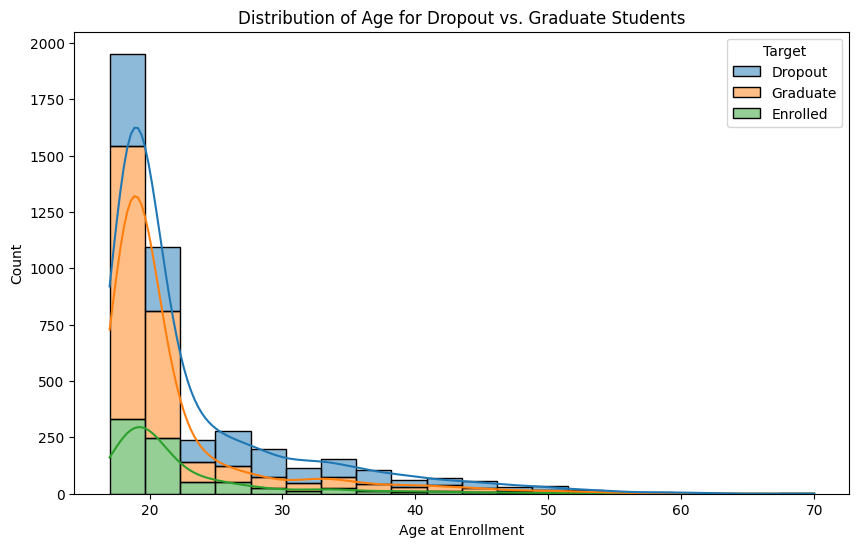
\includegraphics{report_AzadhdhinNedalYunisAlFraijat_files/figure-pdf/fig-age-distr-output-1.png}

}

\caption{\label{fig-age-distr}Distribution of age for dropout and
graduate student}

\end{figure}

Q. v. the sizes of the bins for dropout students differ far less than
the total size for the name of the student.

If the hypothesis about some external factors is correct , the target
variable should be much dependent on previous grades,\\
The datapoint cloud on Table~\ref{fig-points-distr}, however, shows that
this rule has a lot of exceptions.

\begin{figure}

{\centering 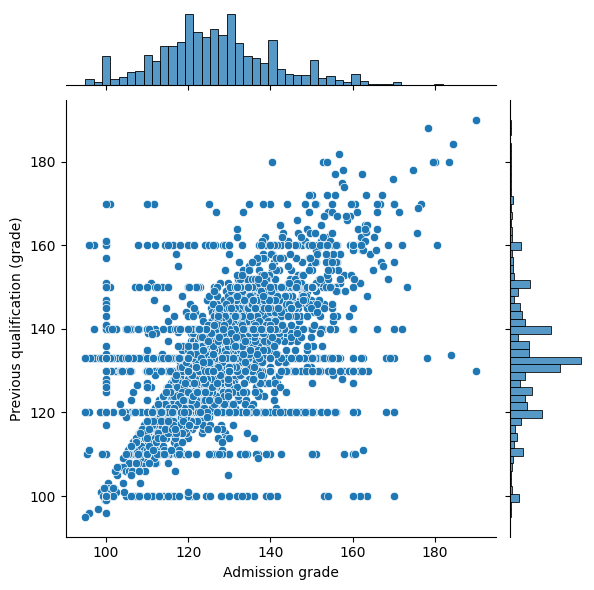
\includegraphics{report_AzadhdhinNedalYunisAlFraijat_files/figure-pdf/fig-points-distr-output-1.png}

}

\caption{\label{fig-points-distr}Joint and marginal distributions of
current admission and previous qualification grades}

\end{figure}

We can draw the following observations:

\begin{itemize}
\item
  The \textbf{distribution of admission grades} is roughly normal with
  most students scoring between \textbf{\emph{120 and 160 marks}}.
\item
  The \textbf{distribution of previous qualifications} (grades) is also
  the same with most of them having grades in between \textbf{\emph{120
  and 160}}.
\item
  There is seen a \textbf{positive correlation} between admission grade
  and previous qualification grade indicating students with higher
  previous qualifications tend to have higher admission grades.
\end{itemize}

The visualizations above, however, were natural for the few quantitative
columns, which show the natural interconnection between the curricularly
accrued units in the 1st and in the 2nd year, which are in turn mostly
unrelated to the admission grade. This is understandable since the
grades are commonly based on the successfulness of the local program and
student's toil, while the students' backgrounds are commonly different
and this puts them into inequitable positions when passing the admission
exams.

In these previous graphs, we considered quantitative columns that are
more or less exogenous to the dataset (e. g. age and the previous
qualification grade are not influenced by the current grade of the
students).

However, the majority of columns of this dataset are qualitative and
they are at least partially endogenous as stem from the decisions during
the study and their consequences. For this, we need to propose a
mechanism of influence, then formulate and test a hypothesis via an
analysis of discriminate groups.

\begin{figure}

{\centering 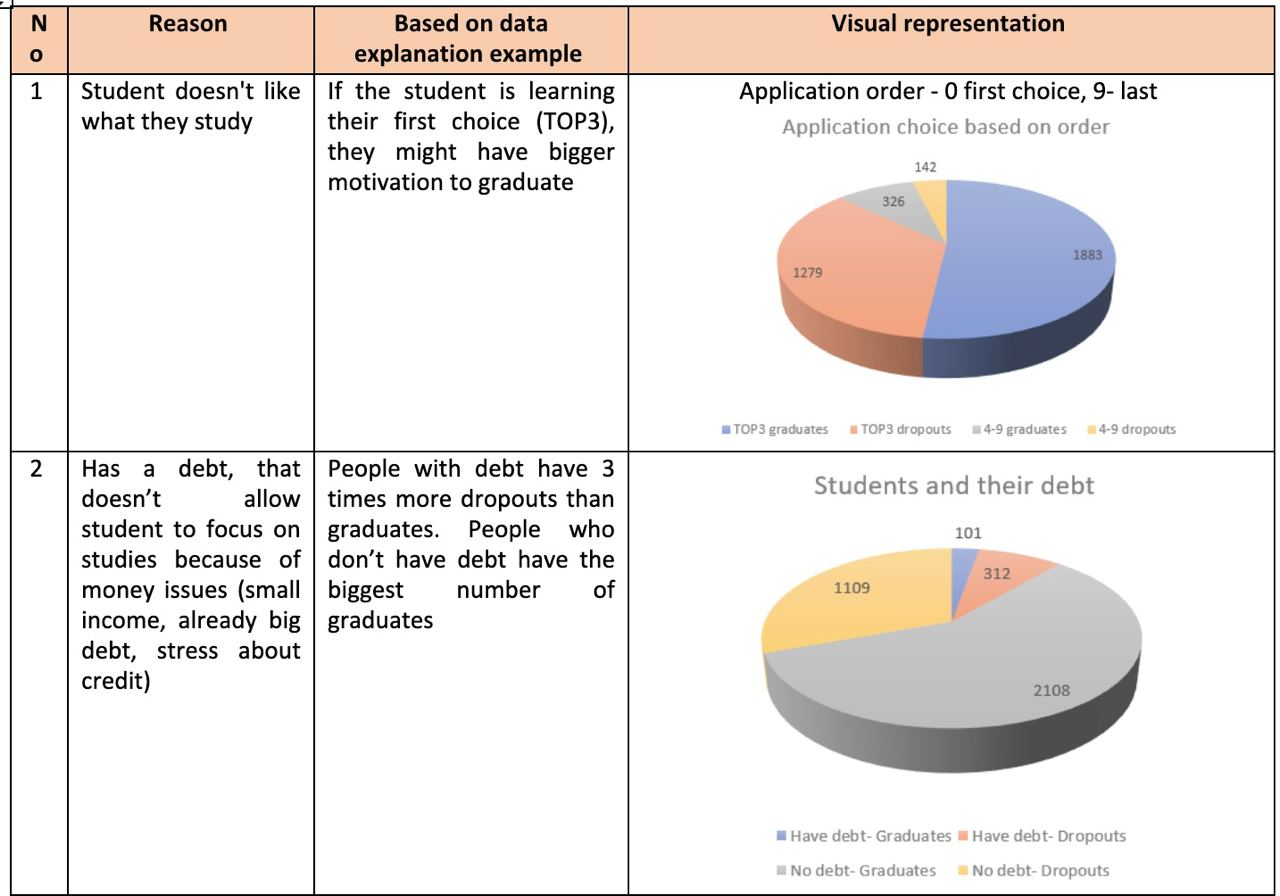
\includegraphics{./figs/reasons-1.jpg}

}

\caption{\label{fig-word-1}Student mobility and financial burden as
indicators and drivers of their motivation and impediments}

\end{figure}

We see on Figure~\ref{fig-word-1} that having debt is always a serious
impediment against studies because it gives wrong incentives towards
directly making money in the short run instead of focusing solely on
one's studies that could aid to make altogether greater money in the
long run.

\begin{figure}

{\centering 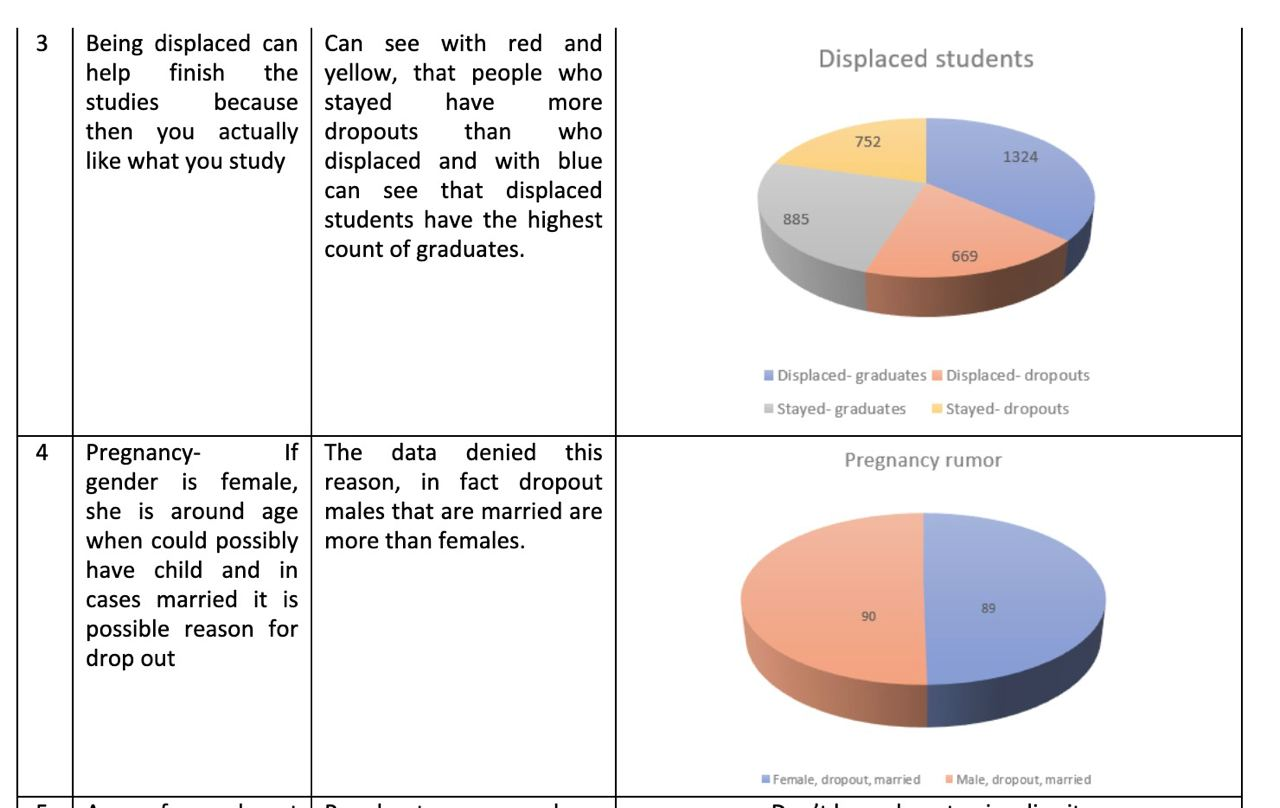
\includegraphics{./figs/reasons2.jpg}

}

\caption{\label{fig-word-2}Student inter-university mobility and health
conditions proxies as indicators and drivers of their motivation towards
learning and impediments (Part 2)}

\end{figure}

We also consider the impact of scholarships and other compensations in
academic support, which should alleviate the complications associated
with adaptations in new environment.

\begin{figure}

{\centering 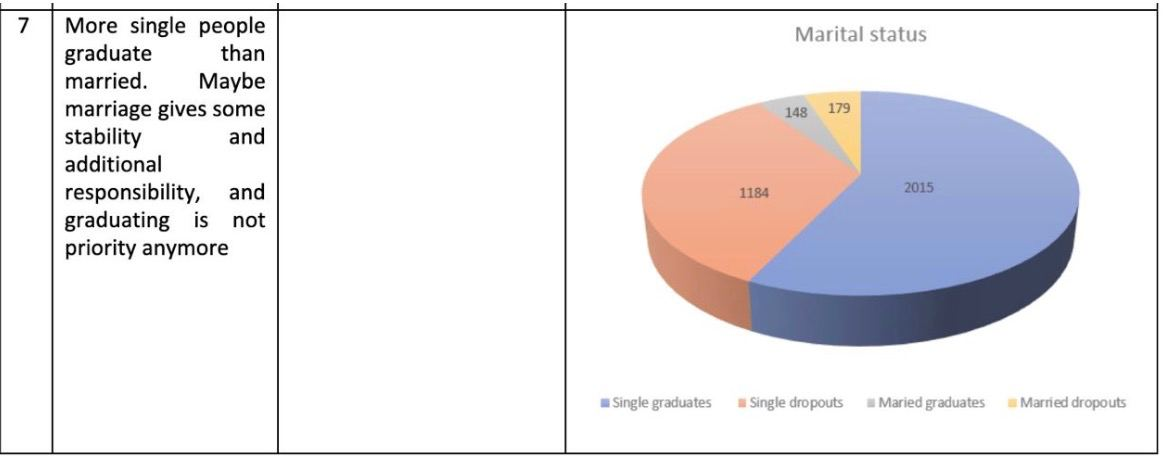
\includegraphics{./figs/reasonsIII.jpg}

}

\caption{\label{fig-word-3}Marital status as distractor from studying}

\end{figure}

In different studies, it is quite common to compare the academic success
of a student with the academic successes of their parents as this has
both direct and indirect effects , s. a. i. e. both are connected to
welfare, but also it can be that there is another channel of knowledge
transmission to the younger generation.

\textbf{Observations :} * The bar chart shows that mother's occupation
is quite influential. This influence is greater the pa's due to
traditional effect, and we distinctly see that students whose mothers
are \enquote*{white collars} dropout significantly more rarely than
those whose mothers are more engaged in physical labor.

\begin{itemize}
\tightlist
\item
  This also may suggest the mother's occupation can influence student
  retention, emphasizing the need for financial support and family
  engagement.
\end{itemize}

\hypertarget{data-correlation-table-quantitative-columns-only}{%
\subsubsection{Data correlation table (quantitative columns
only)}\label{data-correlation-table-quantitative-columns-only}}

\begin{figure}

{\centering 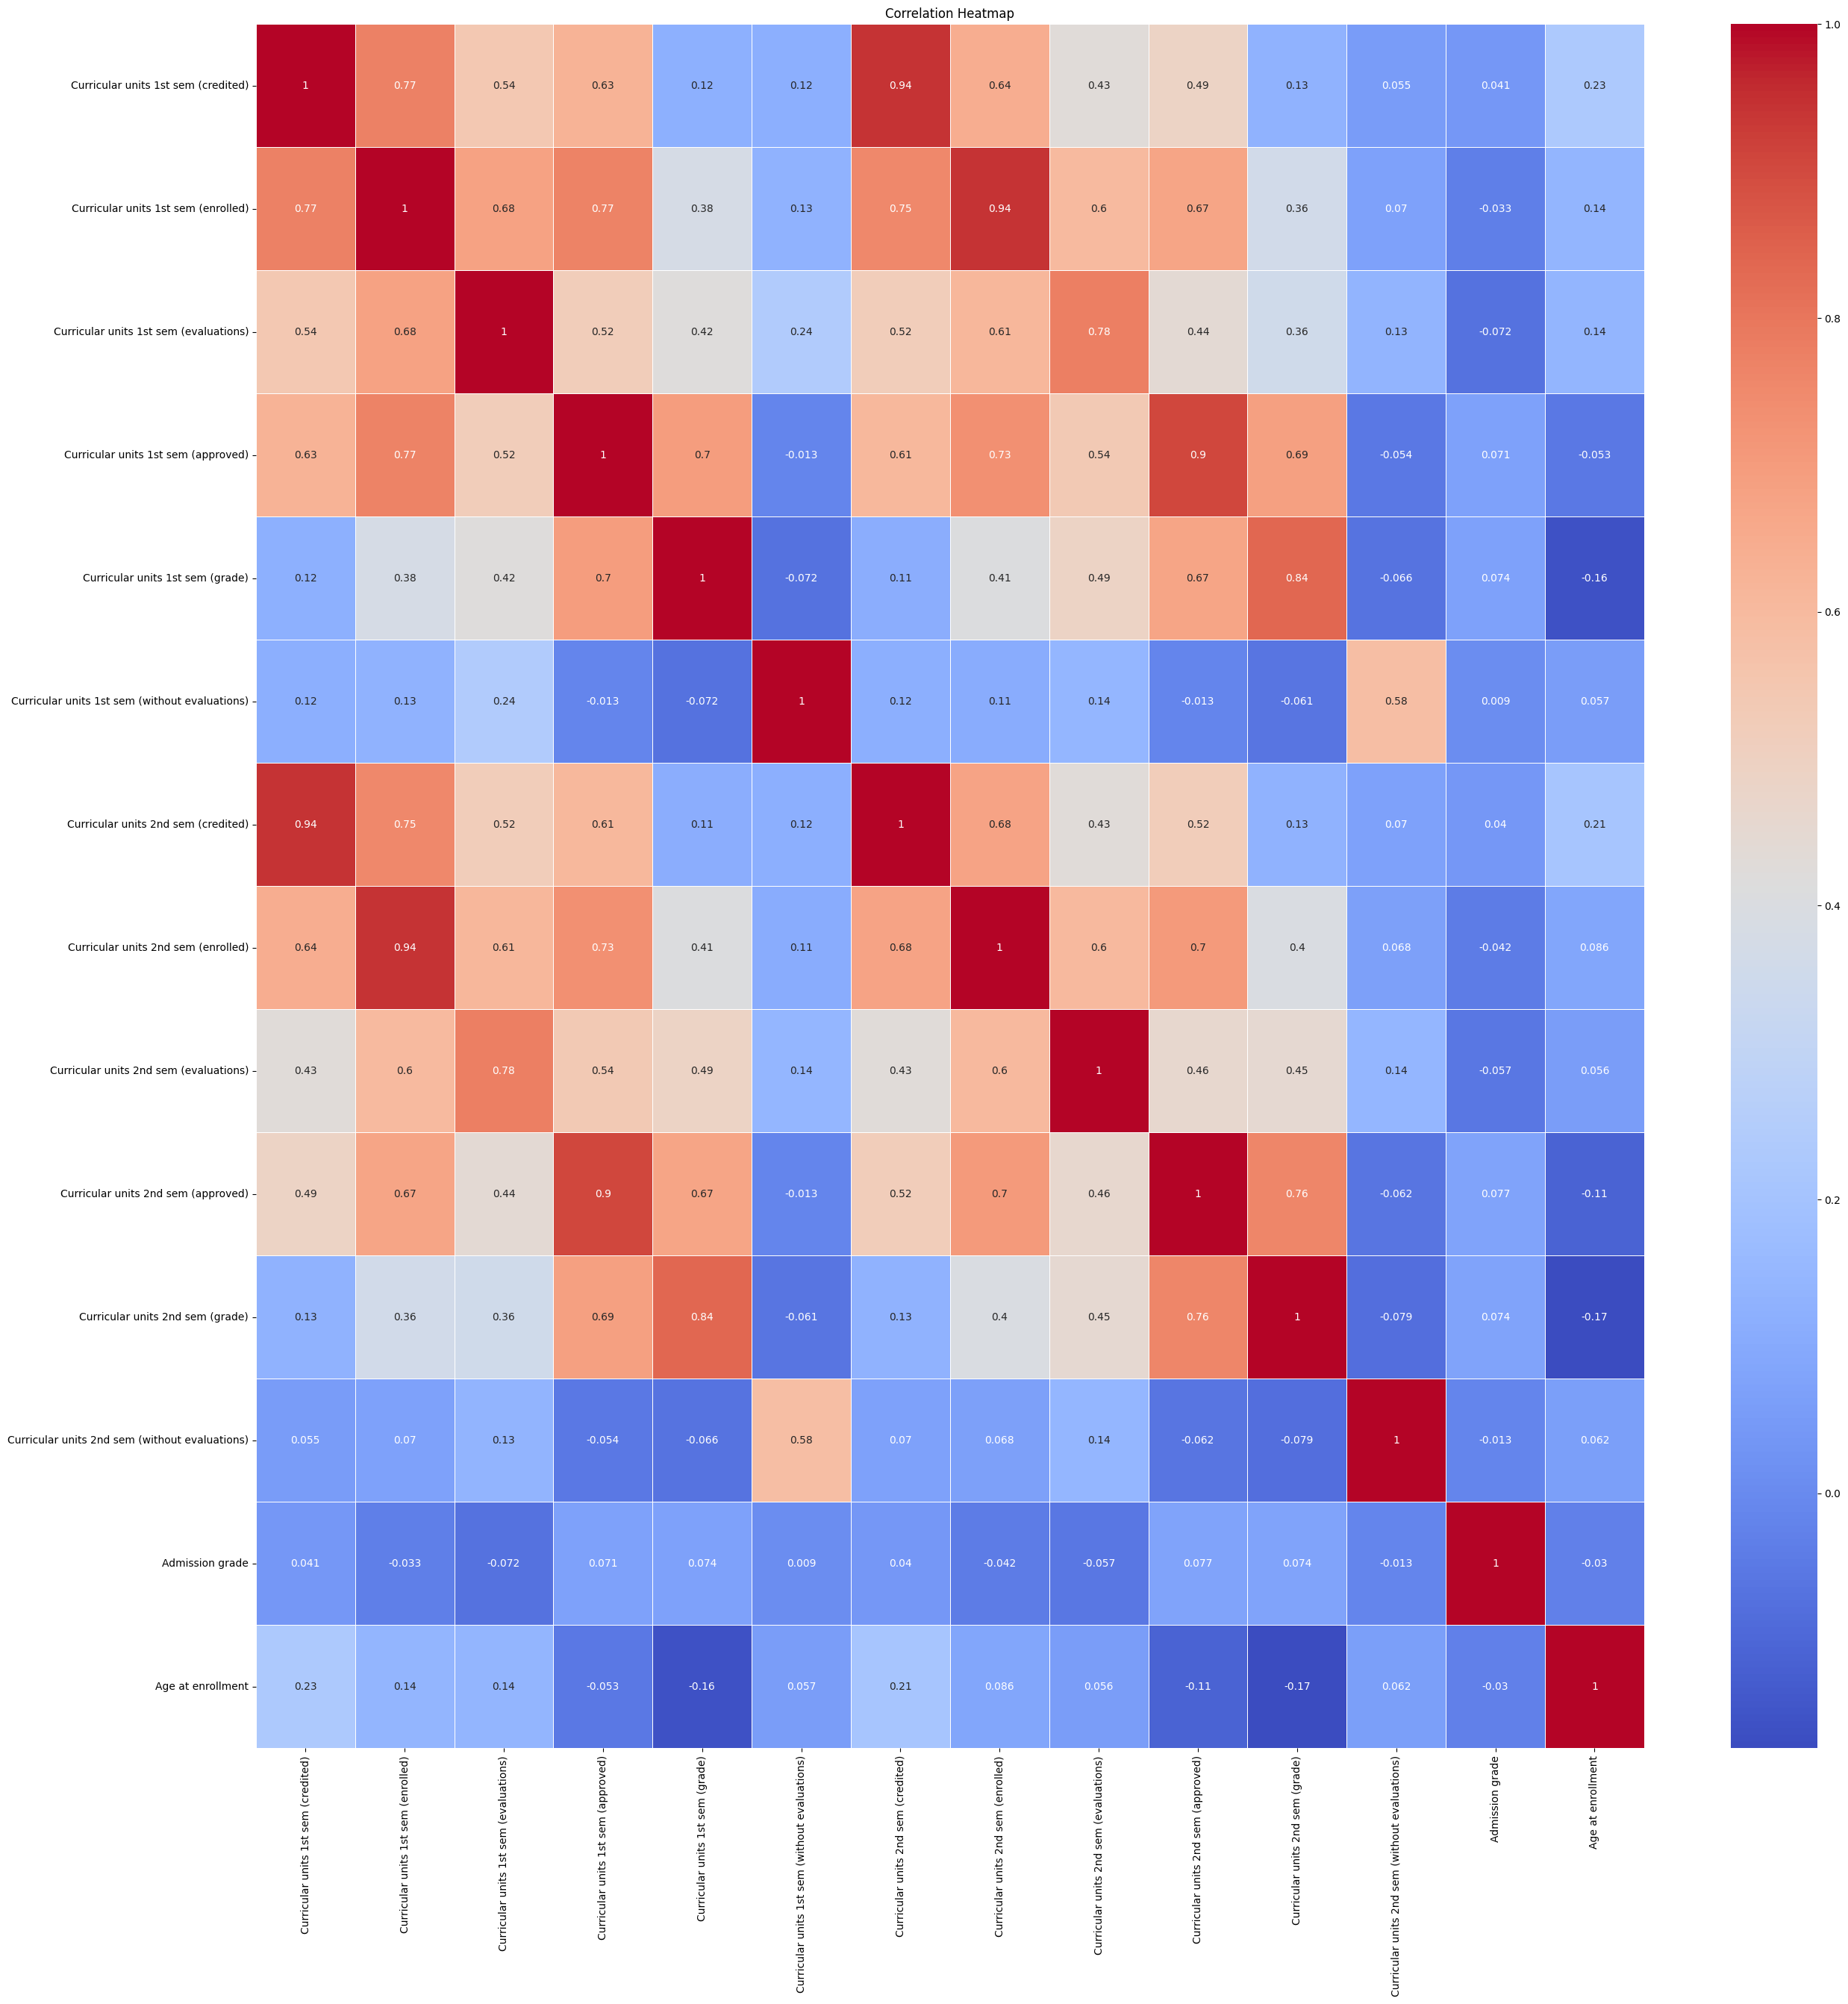
\includegraphics{report_AzadhdhinNedalYunisAlFraijat_files/figure-pdf/fig-correlation-output-1.png}

}

\caption{\label{fig-correlation}Data correlation table (quantitative
columns are represented only since there to compute true correlations
between quantitative columns it is necessary to OHE-encode them, which
would burst no. of columns to many thousands, but the values of the
correlations will be statistically insignificant due to low cardinality
of 90\% of classes)}

\end{figure}

As visible on Figure~\ref{fig-correlation}, there are strong positive
correlation among the curricular units for 1st and 2nd sem that could
suggest that students that are doing well in the first sem will
certainly do well in the upcoming semester. This could suggest that
students with lower curricular units have a higher chance of dropping
out due to their academic preparedness and failing to meet the
requirements and expectations of the study program.

\begin{longtable}[]{@{}llllllllllllllllllllll@{}}
\toprule\noalign{}
& Marital status & Application mode & Application order & Course &
Daytime/evening attendance & Previous qualification & Previous
qualification (grade) & Nacionality & Mother\textquotesingle s
qualification & Father\textquotesingle s qualification & ... &
Curricular units 2nd sem (credited) & Curricular units 2nd sem
(enrolled) & Curricular units 2nd sem (evaluations) & Curricular units
2nd sem (approved) & Curricular units 2nd sem (grade) & Curricular units
2nd sem (without evaluations) & Unemployment rate & Inflation rate & GDP
& Target \\
\midrule\noalign{}
\endhead
\bottomrule\noalign{}
\endlastfoot
0 & 1 & 17 & 5 & 171 & 1 & 1 & 122.0 & 1 & 19 & 12 & ... & 0 & 0 & 0 & 0
& 0.000000 & 0 & 10.8 & 1.4 & 1.74 & Dropout \\
1 & 1 & 15 & 1 & 9254 & 1 & 1 & 160.0 & 1 & 1 & 3 & ... & 0 & 6 & 6 & 6
& 13.666667 & 0 & 13.9 & -0.3 & 0.79 & Graduate \\
2 & 1 & 1 & 5 & 9070 & 1 & 1 & 122.0 & 1 & 37 & 37 & ... & 0 & 6 & 0 & 0
& 0.000000 & 0 & 10.8 & 1.4 & 1.74 & Dropout \\
3 & 1 & 17 & 2 & 9773 & 1 & 1 & 122.0 & 1 & 38 & 37 & ... & 0 & 6 & 10 &
5 & 12.400000 & 0 & 9.4 & -0.8 & -3.12 & Graduate \\
4 & 2 & 39 & 1 & 8014 & 0 & 1 & 100.0 & 1 & 37 & 38 & ... & 0 & 6 & 6 &
6 & 13.000000 & 0 & 13.9 & -0.3 & 0.79 & Graduate \\
... & ... & ... & ... & ... & ... & ... & ... & ... & ... & ... & ... &
... & ... & ... & ... & ... & ... & ... & ... & ... & ... \\
4419 & 1 & 1 & 6 & 9773 & 1 & 1 & 125.0 & 1 & 1 & 1 & ... & 0 & 6 & 8 &
5 & 12.666667 & 0 & 15.5 & 2.8 & -4.06 & Graduate \\
4420 & 1 & 1 & 2 & 9773 & 1 & 1 & 120.0 & 105 & 1 & 1 & ... & 0 & 6 & 6
& 2 & 11.000000 & 0 & 11.1 & 0.6 & 2.02 & Dropout \\
4421 & 1 & 1 & 1 & 9500 & 1 & 1 & 154.0 & 1 & 37 & 37 & ... & 0 & 8 & 9
& 1 & 13.500000 & 0 & 13.9 & -0.3 & 0.79 & Dropout \\
4422 & 1 & 1 & 1 & 9147 & 1 & 1 & 180.0 & 1 & 37 & 37 & ... & 0 & 5 & 6
& 5 & 12.000000 & 0 & 9.4 & -0.8 & -3.12 & Graduate \\
4423 & 1 & 10 & 1 & 9773 & 1 & 1 & 152.0 & 22 & 38 & 37 & ... & 0 & 6 &
6 & 6 & 13.000000 & 0 & 12.7 & 3.7 & -1.70 & Graduate \\
\end{longtable}

In the remaining part, we examine the correlations of purely endogenous
temporal variables. This does not give a scoop about the source of
causation and is not a good predictor, but exhibits an analysis of
autocorrelation inside the quasi-temporal data.

\begin{figure}

{\centering 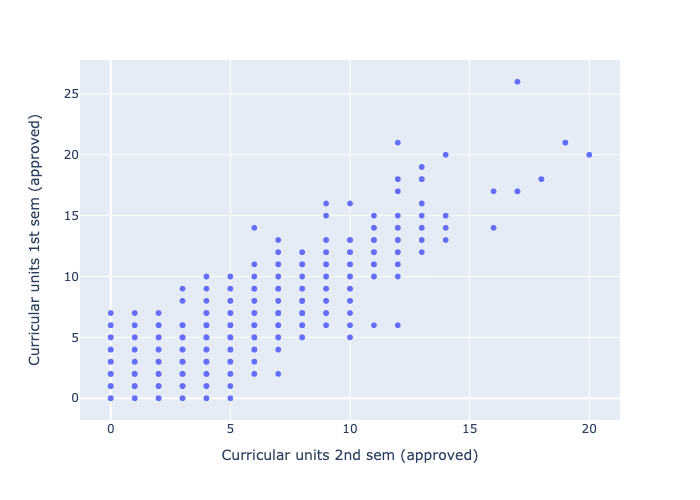
\includegraphics{report_AzadhdhinNedalYunisAlFraijat_files/figure-pdf/fig-cur-units-output-1.png}

}

\caption{\label{fig-cur-units}Vizualization for curricular successively
approved units}

\end{figure}

We can see that the points for the 1st semester and 2nd semester are
correlated which shows that are one's marks are primary drivers of
success and exhibit sizeable correlations

\begin{figure}

{\centering 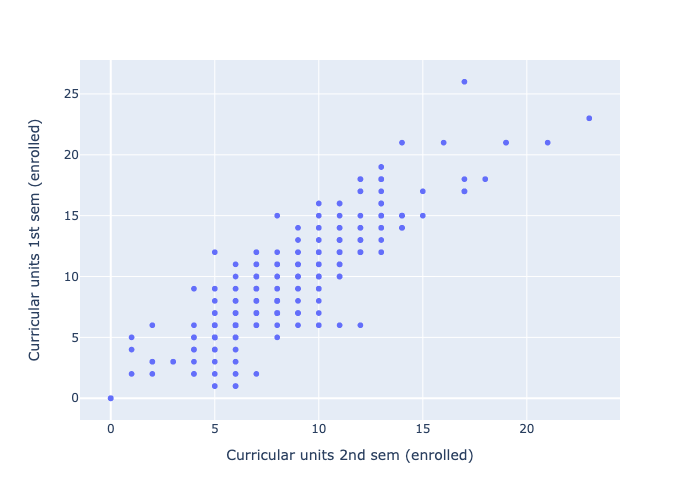
\includegraphics{report_AzadhdhinNedalYunisAlFraijat_files/figure-pdf/fig-cur-units-enrolled-output-1.png}

}

\caption{\label{fig-cur-units-enrolled}Vizualization for curricular
successively enrolled units}

\end{figure}

\begin{figure}

{\centering 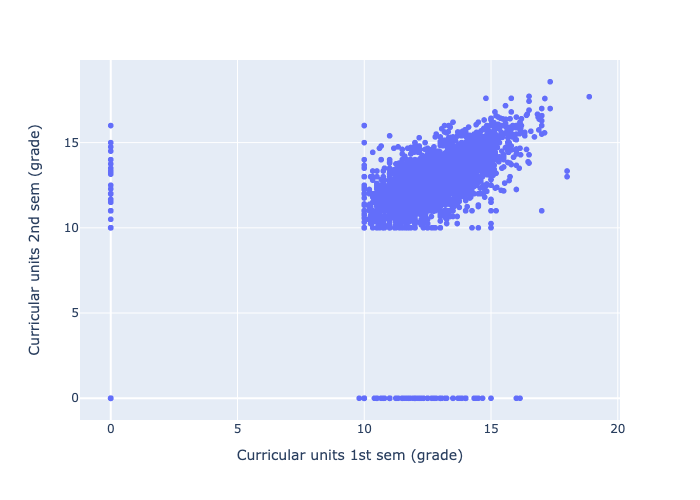
\includegraphics{report_AzadhdhinNedalYunisAlFraijat_files/figure-pdf/fig-cur-grade-output-1.png}

}

\caption{\label{fig-cur-grade}Vizualization of curricular units for the
1st semester}

\end{figure}

\hypertarget{unmentioned-data-issues}{%
\subsubsection{Unmentioned data issues}\label{unmentioned-data-issues}}

While the dataset does not have empty columns , there is some auxiliary
data that could be very appropriate to have together with it. For
example, we have data for years that are many in today's changing
education environment, but there is no open data as proxy for the
conditions in which the students have to study and which influence their
dropout ratios (causing affection or not). Apart from data on
schorlarships, any transitions and their effect (even though hapenned
during reforms in Portugal education field in 2000s-10s) are downplayed.

\hypertarget{sec-data-mining}{%
\subsection{Data Mining}\label{sec-data-mining}}

Now, we need to define our data mining strategy. In the matrix
\ref{fig-correlation} for correlations, we already see high correlations
between many values. Hence, if we (certainly we should) also consider
categorical variables in our data mining analysis, we must reduce the
number of variables because the true dimensionality of the initial space
is too high and virtually all ways of embedding and distance calculation
are too costly and prohibitive given a relatively small amount of
datapoints in this dataset.

In EDA Section~\ref{sec-eda}, we already stressed the issue of class
imbalance. To at least partially recompense for this, we need to perform
SMOTE augmentation of scarcer classes. After dataset is SMOTE-amplified,
our common step would be to dispose of multicollinear columns.\\
High dimensionality prevents intuitive DBSCAN threshold setting and some
inferior algorithms as TSNE. Hence, although not considering distal
non-linear data structures, we reduce the dimensionality via principal
component analysis.

After we perform the PCA, the estimators from various standard families
are idependently fine-tuned, by mean F1 measure, the model that is most
precise in predicting the outcome is rendered. We confer some other
renowned metrics for the best model . In total, we consider 3 different
types of models for classification (logical, linear separative, linear
generative), implying algorithms of various \enquote*{difficulty}
levels, including 3 boostings: LGBoosting, XGBoosting (gbc), Catboost,
Random Forest, a Decision Tree as well as linear discriminate analysis
and logistic regression. We test models against each other and against
dummy classifier. The results of the best models are given in
leaderboard below in Table~\ref{tbl-leaderboard}.

\begin{verbatim}
<IPython.core.display.HTML object>
\end{verbatim}

\hypertarget{tbl-leaderboard}{}
\begin{longtable}[]{@{}llllllllll@{}}
\toprule\noalign{}
~ & Model & Accuracy & AUC & Recall & Prec. & F1 & Kappa & MCC & TT
(Sec) \\
\midrule\noalign{}
\endfirsthead
\toprule\noalign{}
~ & Model & Accuracy & AUC & Recall & Prec. & F1 & Kappa & MCC & TT
(Sec) \\
\midrule\noalign{}
\endhead
\bottomrule\noalign{}
\endlastfoot
catboost & CatBoost Classifier & 0.7290 & 0.8626 & 0.7290 & 0.7099 &
0.7150 & 0.5443 & 0.5491 & 1.8750 \\
gbc & Gradient Boosting Classifier & 0.7293 & 0.8674 & 0.7293 & 0.7124 &
0.7147 & 0.5426 & 0.5494 & 0.6640 \\
lightgbm & Light Gradient Boosting Machine & 0.7248 & 0.8591 & 0.7248 &
0.7044 & 0.7092 & 0.5357 & 0.5413 & 0.8520 \\
rf & Random Forest Classifier & 0.7255 & 0.8644 & 0.7255 & 0.7041 &
0.7088 & 0.5357 & 0.5420 & 0.1450 \\
lda & Linear Discriminant Analysis & 0.7190 & 0.8560 & 0.7190 & 0.7047 &
0.6984 & 0.5163 & 0.5310 & 0.0370 \\
ridge & Ridge Classifier & 0.7125 & 0.0000 & 0.7125 & 0.6846 & 0.6676 &
0.4912 & 0.5196 & 0.0300 \\
dt & Decision Tree Classifier & 0.6237 & 0.7070 & 0.6237 & 0.6283 &
0.6251 & 0.3907 & 0.3914 & 0.0570 \\
lr & Logistic Regression & 0.4754 & 0.5142 & 0.4754 & 0.3960 & 0.4313 &
0.0909 & 0.0956 & 0.5740 \\
dummy & Dummy Classifier & 0.4994 & 0.5000 & 0.4994 & 0.2494 & 0.3326 &
0.0000 & 0.0000 & 0.0670 \\
\caption{\label{tbl-leaderboard}Results of fitting estimators of
different families}\label{T_967cf}\tabularnewline
\end{longtable}

\begin{verbatim}
<IPython.core.display.HTML object>
\end{verbatim}

\begin{figure}

{\centering 

\begin{figure}

{\centering 

\begin{verbatim}
<IPython.core.display.HTML object>
\end{verbatim}

}

\caption{Stylized ROC curves for the Catboost Model}

\end{figure}

\begin{figure}

{\centering 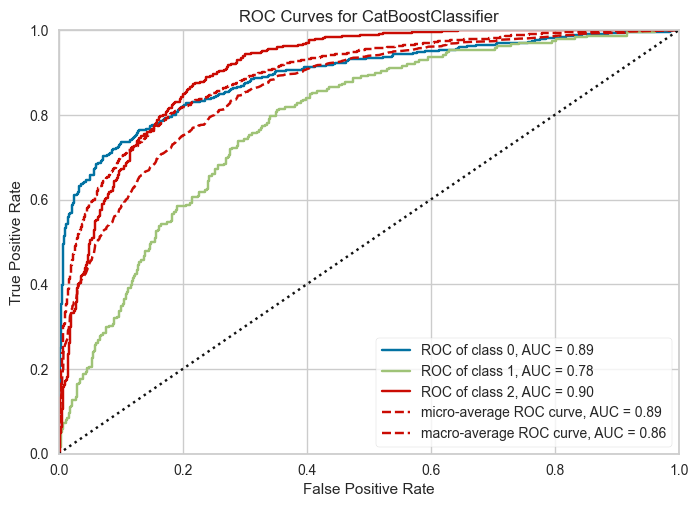
\includegraphics{report_AzadhdhinNedalYunisAlFraijat_files/figure-pdf/fig-rocauc-output-2.png}

}

\end{figure}

}

\caption{\label{fig-rocauc}\textbf{?(caption)}}

\end{figure}

\begin{verbatim}
Requirement already satisfied: graphviz in /opt/homebrew/Caskroom/miniconda/base/lib/python3.11/site-packages (0.20.1)
\end{verbatim}


\includegraphics{report_AzadhdhinNedalYunisAlFraijat_files/mediabag/report_AzadhdhinNedalYunisAlFraijat_files/figure-pdf/cell-55-output-1.pdf}

\begin{verbatim}
(Pipeline(memory=Memory(location=None),
          steps=[('label_encoding',
                  TransformerWrapperWithInverse(exclude=None, include=None,
                                                transformer=LabelEncoder())),
                 ('numerical_imputer',
                  TransformerWrapper(exclude=None,
                                     include=['Marital status',
                                              'Application mode',
                                              'Application order', 'Course',
                                              'Daytime/evening attendance',
                                              'Previous qualification',
                                              'Previous qualification (gra...
                                                     iterated_power='auto',
                                                     n_components=10,
                                                     n_oversamples=10,
                                                     power_iteration_normalizer='auto',
                                                     random_state=None,
                                                     svd_solver='auto', tol=0.0,
                                                     whiten=False))),
                 ('clean_column_names',
                  TransformerWrapper(exclude=None, include=None,
                                     transformer=CleanColumnNames(match='[\\]\\[\\,\\{\\}\\"\\:]+'))),
                 ('trained_model',
                  <catboost.core.CatBoostClassifier object at 0x295e30790>)],
          verbose=False),
 'models/SOTA_catboost.pkl')
\end{verbatim}

Thus, the best model by F1 measure is CatBoostClassifier, which is
renowned for scoring fairly well on tabular data, while ordinary GBC is
the most second to prime and the most robust one, featuring best
conventional recall, accuracy, and precision metrics. The

However, while all top models in Table~\ref{tbl-leaderboard} demonstrate
significant improvement over a dummy classifier and other simplistic
models such as Logistic Regression, the scores are still which indicates
that reduction of dimensionality, which is inevitable under given class
imbalance, has come at a price of variance loss, or, alternatively, all
the covariates do not explain sufficiently well the outcome of studies:
in academic success, as in life, a lot depends on the proper
characteristics of a person which are difficult to elicit and much is
undetermined.

\hypertarget{conclusion}{%
\subsection{\texorpdfstring{\textbf{Conclusion}}{Conclusion}}\label{conclusion}}

\begin{quote}
With this analysis, we have some valuable insights some crucial factors
like Academic support, socioeconomic factors, previous qualifications,
and others play a significant role in student retention.
\end{quote}

\begin{quote}
The observed patterns imply a lot to stress in the lives of students and
their associates. First, we strive to insentivize parents to improve
their labour efficiency and pursue greater carreer so that ultimately
they could dedicate more time to their children's education, and
proactively stir their self-propelled interest. Additionally, we could
provide financial assistance to those who are struggling to pay with if
this is contemporaneous with a significant degradation in their
university marks, as this subrogates the stimuli for a person in an age
where they are most perceptive to knowledge and is a good predictor of a
dropout. Also importantly, we could teach the students, especially going
on their second studies, that it is quite unlikely that they are going
to get high grades or exit the university without proper time management
and confirmation that they assign top priority to their studies. They
are also advised to make that clear to all their relatives and
stakeholders who might underestimate the effects of such a change.
Although this could result in a reduction of enthusiastic entrants, this
would increase at least the KPI of retention and arguably also increase
the KPI on number of diplomas issued, because with fewer but more
motivated students the university would have more time to dedicate to
most obstinate pending alumni.
\end{quote}

\begin{quote}
Addressing these factors carefully can effectively lead to dropout rates
reduction and improve overall student outcomes
\end{quote}


\printbibliography


\end{document}
